\quad In this section, we carry out empirical analysis on two real world cascades datasets to show that the assumption of constant influence strength does not hold. We then provide a method to estimate the popularity of the information under propagation empirically from the observed cascades. 

\subsection{Existence of influence strength heterogeneity}
\quad In many network inference models, the influence strength parameter $\alpha_{u,v}$ models the speed of diffusion, namely the time it takes for the information to propagation from user $u$ to $v$.  We empirically estimate the average diffusion speed as the inverse of delay time in two real world cascade datsets, Sina microblog and US Patent to show the heterogeneity of influence strength. \xhcomment{Sina dataset contains the hyper-links such as user $u$ reposts one of $v$'s microblog with delay $t_u-t_v$. Patent dataset contains citation links between patent products.}

The estimation process is as follows: we first normalize the span of each cascade to $[0,1]$ and split the interval into ten bins. We treat each bin as one stage of the diffusion process. We estimate the average diffusion speed in each bin as the inverse of delay time $\frac{1}{\Delta_t}$ using the available explicit following information in the datasets. \xhcomment{What is the unit of y-axis? Is it the diffusion speed after normalization? Ans: I think the inverse of diffusion speed is normalized but diffusion speed isn't. As the unit of y-axis contains normalization value, I'm confused about how to express the unit $\sim\sim$} The results on two cascades from each dataset is shown in Figure \ref{fig:PatentHetero}. 
\begin{figure}[h]
\subfigure[Cascades of Sina Microblog dataset]{\centerline{
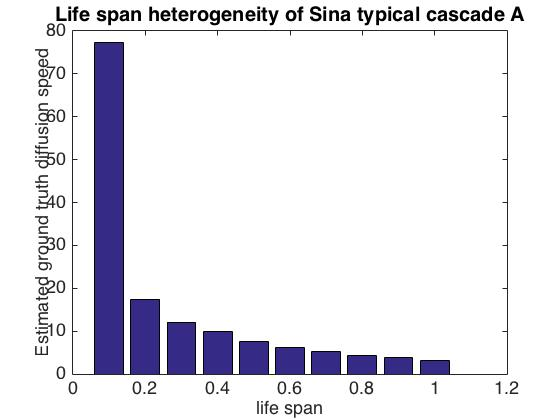
\includegraphics[width=0.55\linewidth]{figures/SinaA.jpg}
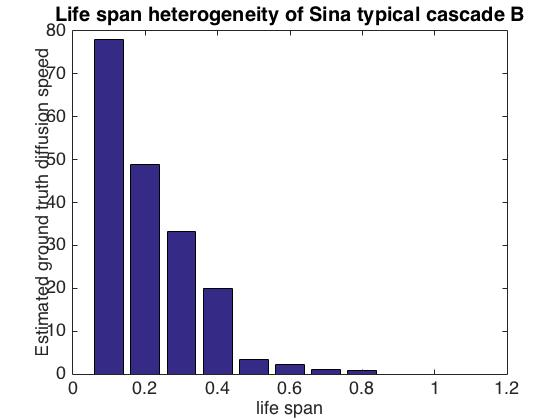
\includegraphics[width=0.55\linewidth]{figures/SinaB.jpg}}}
\subfigure[Cascades of U.S. Patent dataset]{\centerline{
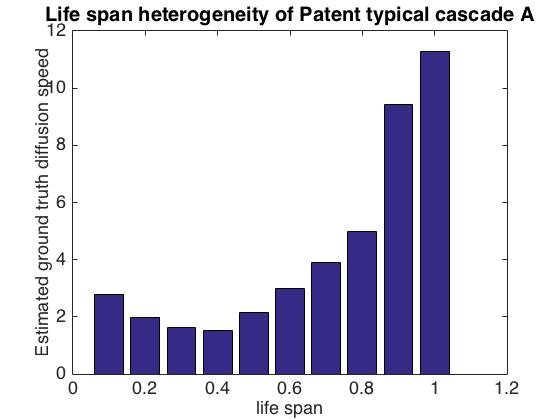
\includegraphics[width=0.55\linewidth]{figures/PatentA.jpg}
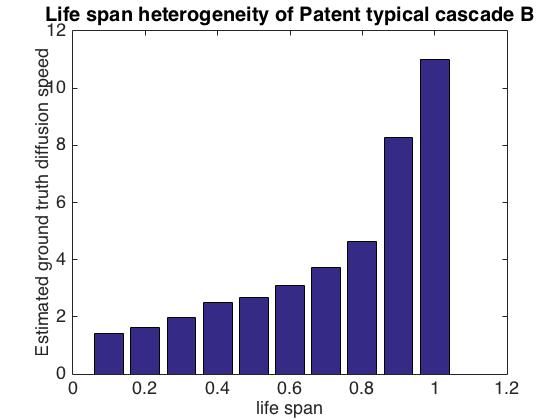
\includegraphics[width=0.55\linewidth]{figures/PatentB.jpg}}}
\caption{The diffusion speed in different stages of diffusion process in two real world datasets. \xhcomment{Could we provide name for each cascade? link the story in microblog and the porduction in patent.  Ans: I'm afraid there is no record in Sina dataset indicating the content of micro-blog; raw data of Patent contains the class of product, such as planting, Jewelry, Bridges, but there can be several different patent classes in a cascade, as one may cite to some patent products in other fields.}}\label{fig:PatentHetero}
\end{figure}

The results clearly demonstrate the deviation from the assumption of constant diffusion speed. Another interesting observation is that the how the diffusion speed depends on the diffusion stages varies dramatically over different cascades and datasets. For the microblog datasets, usually the diffusion speed decrease when the story under propagation becomes stale and less interesting as time elapses. On the contrary, in the patent datsets, newly invented product gradually gains popularity leading to increment in the diffusion speed. 

%It implies that assuming particular functional form of the popularity for all cascades may lead to inaccurate estimation. As a result, we propose to represent the cascade popularity $\DS(t)$ as a piece-wise constant function. Assume we split the normalized span of the cascade into $k$ bins with $t_0=0 < t_1 < \ldots < t_K = 1$. We have $\DS(t) = \DS_i$ if $t\in[t_{i-1}, t_i]$.

%We make an interesting analysis of message's diffusion speed on 2 real world datasets: Sina microblog and U.S. patent. We normalize the activation times with Min-Max method and divide the time length of cascade into several periods.
%As diffusion speed is unmeasurable, we compute the $\frac{1}{\overline{\Delta t}}$ in each life span that is proportion to the ground truth diffusion speed. As in Figure \ref{fig:PatentHetero}, the maximum of $\frac{1}{\overline{\Delta t}}$ reaches 80 in Sina and about 12 in Patent dataset, while the minimum approaches 0. There is distinct difference of diffusion speed in different life span. However, former algorithms have not taken this into consideration. They assume that the coefficient of $\Delta t$'s distribution which controls diffusion speed does not change with time. We believe the life span heterogeneity is a key point to re-understand network inference problem.

%==========================
\subsection{Approximation popularity with number of activation}
\quad Direct estimation of average diffusion speed requires the diffusion pathway which is usually not available in real world datasets. It is even harder to estimate the average activation probability from observed cascades. As a result, we have to seek approximation for the true popularity for different stages in the diffusion process. In the work, we find the total number of activated nodes in each stage of the diffusion process as a good surrogate for the average diffusion speed or the activation probability as a measure for the popularity level. 

Let $I^c(t)$ be the number of activated nodes in cascades $c$ till time $t$. We approximate the popularity level with the following formula:
$$
\DS^c(t) = (I^c(t+\frac{L}{2}) - I^c(t-\frac{L}{2})) / I^c(1).
$$
That is to say, the estimated popularity level at time $t$ is ratio of nodes activated in the windows of length $L$, $[t-\frac{L}{2}, t+\frac{L}{2}]$. 

We carry out experiments to show that the proposed surrogate popularity level is a valid approximation. \xhcomment{We sort all cascades descendingly by activation number and select the top 80 cascades in Patent dataset and top 50 cascades in Sina dataset}. For each cascade, we first normalize the time span to $[0,1]$ and split it into $K$ bins\xhcomment{(we use $k=10$ in this part)}. The true popularity level is assumed to be constant as the average diffusion speed estimated from the particular cascade. We compare the true popularity level and the surrogate popularity at each activation time $t_a$ by computing the Pearson correlation for each cascade. The distribution on the correlation coefficient on the two datasets are shown in Table \ref{tab:Corre}. More than 60\% cascades and 80\% cascades in Patent and Sina microblog dataset respective have correlation coefficient $r>0.6$ with the true popularity level.   


%We show the validity of this approach by empirically calculating the correlation. We select 80 long cascades in Patent dataset and 50 long cascades in Sina dataset. As in Table \ref{tab:Corre}, we use Evans's (1996) interpretation for r coefficient to describe the strength of correlation. 65\% of Patent cascades and 90\% of Sina cascades present strong or very stronger correlation. Our approach of calculating activated nodes number can reflect the level of diffusion speed to a large extent.
\begin{table}[H]
\caption{Correlation coefficients between ground truth diffusion speed and the number of activated nodes in time unit.}
\begin{tabular}{c|c|c|c}
 coefficient range & strength & pct. Patent & pct. Sina \\
\hline
.00-.19 & very weak & 0.05 & 0.02\\
.20-.39 & weak & 0.125 & 0.02\\
.40-.59 & moderate & 0.175 & 0.06\\
.60-.79 & strong & 0.3 & 0.08\\
.80-1.0 & very strong & 0.35 & 0.82\\
\end{tabular}\label{tab:Corre}
\end{table}